\documentclass[11pt,oneside]{article}
\usepackage[utf8]{inputenc}
\usepackage[a4paper,top=2cm,left=2cm,right=2cm,bottom=2cm]{geometry}
\usepackage{import}
\usepackage[T1]{fontenc}
\usepackage[german,ngerman]{babel}
\usepackage[table]{xcolor}
\usepackage{amsthm, esvect}
\usepackage{mathtools}
\RequirePackage{amssymb, amsfonts, amsmath, latexsym, verbatim, xspace}
\usepackage{systeme}
\usepackage{multicol}
\usepackage{multirow}
\usepackage{framed}
\usepackage{array}
\usepackage{ragged2e}
\usepackage{graphicx}
\usepackage{pdflscape}
\usepackage{epstopdf}
\usepackage{booktabs}
\usepackage{pdfpages}
\usepackage{float} % Allows putting an [H] in \begin{figure} to specify the exact location of the figure
\usepackage{wrapfig} % Allows in-line images such as the example fish picture
\usepackage{tikz, graphicx} % tikz
\usepackage[position=top]{subfig}
\usepackage[bookmarks=true]{hyperref}%Links
\usepackage{enumerate}
\usepackage{enumitem}
\usepackage[german,ruled,vlined,linesnumbered,algosection]{algorithm2e}
\usepackage[labelfont=sf]{caption}
\usepackage{lmodern}
\usepackage{lscape}
\usepackage{tabularx}
\usepackage{systeme}
\usepackage{hhline}
\usepackage{subfiles}
\usepackage{stackengine}
\usepackage{setspace}
\usepackage{MnSymbol}
\usepackage{tcolorbox}
\usepackage{bbm}
\usepackage{url}
\usepackage{xparse}
\usepackage{sectsty}
\usepackage{array}
\usepackage{ragged2e}
\usepackage{listings} %Stellt Code-Snippets sauber dar

% definiert die Sprache
\selectlanguage{German}

% add command for different dates in Swiss fashion
\newcommand{\monthwordlong}[1]{\ifcase#1 \or Januar\or Februar\or März\or April\or Mai\or Juni\or Juli\or August\or September\or Oktober\or November\or Dezember\fi}
\newcommand{\monthwordshort}[1]{\ifcase#1\or Jan\or Feb\or Mar\or Apr\or Mai\or Jun\or Jul\or Aug\or Sept\or Okt\or Nov\or Dez\fi}
\newcommand{\datelong}{\number\day.\:\monthwordlong{\the\month}\:\number\year}
\newcommand{\dateshort}{\number\day.\:\monthwordshort{\the\month}\:\number\year}

% define color of links inside a text
\definecolor{linkblue}{RGB}{0, 0, 80}
\definecolor{plotblue}{RGB}{100, 100, 255}
\definecolor{myblue}{RGB}{8,164,214}
\definecolor{myred}{RGB}{143,42,41}
\definecolor{forestgreen}{RGB}{34,139,34}
\definecolor{highdive}{RGB}{10,169,194}
\definecolor{charcoal}{RGB}{74,74,74}
\hypersetup{
	colorlinks=true,
	linkcolor=linkblue,
	filecolor=magenta,
	urlcolor=plotblue,
	citecolor=linkblue,
	pdfpagemode=FullScreen,
}


\lstdefinestyle{mystyle}{ % definiert den style des Code-Snippets
	%backgroundcolor=\color{backcolour},
	%commentstyle=\color{codegreen},
	%keywordstyle=\color{magenta},
	%numberstyle=\tiny\color{codegray},
	%stringstyle=\color{codepurple},
	basicstyle=\ttfamily\footnotesize,
	breakatwhitespace=false,
	breaklines=true,
	captionpos=b,
	keepspaces=true,
	%numbers=left,
	%numbersep=5pt,
	showspaces=false,
	showstringspaces=false,
	showtabs=false,
	tabsize=4
}
\lstset{style=mystyle}
\usepackage{fancyhdr}

\tcbuselibrary{breakable,skins}
\usetikzlibrary{mindmap,trees}
\newlength\tindent
\setlength{\tindent}{\parindent}
\setlength{\parindent}{0pt}
\renewcommand{\indent}{\hspace*{\tindent}}

\makeatletter
\def\ifEmpty#1{\def\@temp{#1}\ifx\@temp\@empty}
\makeatother

\sectionfont{\underline}
\usetikzlibrary{arrows, petri, topaths, graphs}


% =================== BEISPIEL ====================
\theoremstyle{definition}
\newtheorem{beispiel}{Beispiel}
\renewcommand{\thebeispiel}{\arabic{beispiel}}

% =================== AUFGABE =====================
\newcounter{aufg}[section] % Zähler für die Umgebungen

\newenvironment{aufgabe}[1][]{%
    \refstepcounter{aufg}% Inkrementiere den Zähler
    \begin{tcolorbox}[%
        enhanced,
        overlay unbroken and first={\mytitleaufg[#1]}, % Titelleiste mit Icons wird nicht über Seite gebrochen
        colframe=black,
        boxrule=0pt,
        breakable,
        top=15pt,
        before=\vskip18pt,
    ]
}{%
    \end{tcolorbox}
}

\newcommand{\mytitleaufg}[1][]{% Definiert die Titelleiste und Icons
    \node[fill=black!20,
        rounded corners,
        draw=black,
        text=black,
        line width=1pt,
        inner sep=4pt,
        anchor=west,
        xshift=12pt]
        at (frame.north west){\bfseries Aufgabe \thesection.\theaufg.\ifEmpty{#1}\else\emph{ (#1)}\fi}; % Titel, letzter Teil mit ifempty testet ob #1 leer und macht Klammern und Titel, falls Titelargument übergeben wird bzw. falls #1 leer erscheint nichts - auch keine Klammern

    \node[% Icon
        rounded corners,
        text=black,
        fill=black,
        line width=0pt,
        inner sep=3pt,
        anchor=west,
        xshift=5pt,
        % yshift=-35pt
        ]
        at (frame.north east){
\includegraphics[width=24pt]{../../../Header/Icons/aufgabeicon.png}};
}

% =================== DEFINITION ==================
\newcounter{def}[section] % Zähler für die Umgebungen

\newenvironment{definition}[1][]{%
    \refstepcounter{def}% Inkrementiere den Zähler
    \begin{tcolorbox}[%
        enhanced,
        drop shadow southeast,
        overlay unbroken and first={\mytitledef[#1]}, % Titelleiste mit Icons wird nicht über Seite gebrochen
        colback=blue!5!white,
        colframe=blue!75!black,
        boxrule=2pt,
        breakable,
        top=15pt,
        before=\vskip18pt,
    ]
}{%
    \end{tcolorbox}
}

\newcommand{\mytitledef}[1][]{% Definiert die Titelleiste und Icons
    \node[fill=blue!40!white,
        rounded corners,
        draw=black,
        text=black,
        line width=1pt,
        inner sep=4pt,
        anchor=west,
        xshift=12pt]
        at (frame.north west){\bfseries Definition \thesection.\thedef.\ifEmpty{#1}\else\emph{ (#1)}\fi}; % Titel, letzter Teil mit ifempty testet ob #1 leer und macht Klammern und Titel, falls Titelargument übergeben wird bzw. falls #1 leer erscheint nichts - auch keine Klammern

    \node[% Icon
        rounded corners,
        text=black,
        fill=black,
        line width=0pt,
        inner sep=3pt,
        anchor=west,
        xshift=5pt,
        % yshift=-35pt
        ]
        at (frame.north east){
\includegraphics[width=24pt]{../../../Header/Icons/definitionicon.png}};
}

% =================== NOTATION ====================
\newcounter{nota}[section] % Zähler für die Umgebungen

\newenvironment{notation}[1][]{%
    \refstepcounter{nota}% Inkrementiere den Zähler
    \begin{tcolorbox}[%
        enhanced,
        drop shadow southeast,
        colback=yellow!5!white,
        colframe=yellow!75!black,
        overlay unbroken and first={\mytitlenota[#1]},   % Titelleiste mit Icons wird nicht über Seite gebrochen
        boxrule=2pt,
        breakable,
        top=15pt,
        before=\vskip18pt,
    ]
}{%
    \end{tcolorbox}
}

\newcommand{\mytitlenota}[1][]{% Definiert die Titelleiste und Icons
    \node[fill=yellow!40!white,,
        rounded corners,
        draw=black,
        text=black,
        line width=1pt,
        inner sep=4pt,
        anchor=west,
        xshift=12pt]
        at (frame.north west){\bfseries Notation \thesection.\thenota.\ifEmpty{#1}\else\emph{ (#1)}\fi}; % Titel, letzter Teil mit ifempty testet ob #1 leer und macht Klammern und Titel, falls Titelargument übergeben wird bzw. falls #1 leer erscheint nichts - auch keine Klammern

    \node[% Icon
        rounded corners,
        text=black,
        fill=black,
        line width=0pt,
        inner sep=3pt,
        anchor=west,
        xshift=5pt,
        % yshift=-35pt
        ]
        at (frame.north east){
\includegraphics[width=24pt]{../../../Header/Icons/definitionicon.png}};
}

% =================== SATZ ========================
\newcounter{satz}[section]  % creates a counter and resets it after each chapter

\newenvironment{satz}[1][]{   % Hauptbox mit Satz drin
    \refstepcounter{satz}
    \begin{tcolorbox}[%
        enhanced,
        colback=red!5!white,
        fuzzy halo=2mm with gray,
        colframe=red!75!black,
        overlay unbroken and first={\mytitlesatz[#1]},   % Titelleiste mit Icons wird nicht über Seite gebrochen
        boxrule=2pt,
        breakable,
        top=15pt,
        before=\vskip18pt,
    ]
}{%
    \end{tcolorbox}
}

\newcommand{\mytitlesatz}[1][]{                     % Macht Titelbox und Icons
   \node[fill=red!90!white,
      rounded corners,
      draw=black,,
      text=black,
      line width=1pt,
      inner sep=4pt,
      anchor=west,
      xshift=12pt]
   at (frame.north west){\bfseries Satz \thesection.\thesatz.\ifEmpty{#1}\else\emph{ (#1)}\fi};  % Titel, letzter Teil mit ifx testet ob #1 leer und macht Klammern und Titel, falls Titelargument übergeben wird bzw.  falls #1 leer erscheint nichts - auch keine Klammern

 \node[ % Icon
      rounded corners,
      text=black,
      fill=black,
      line width=0pt,
      inner sep=3pt,
      anchor=west,
      xshift=5pt,
%     yshift=-35pt
]
   at (frame.north east){ 
\includegraphics[width=24pt]{../../../Header/Icons/satzicon.png} };
}

% =================== BEWEIS ======================
\newenvironment{beweis}[1][]{
    \begin{tcolorbox}[
        enhanced,
        overlay unbroken and first={\mybeweis[#1]},     % Titelleiste mit Icons wird nicht über Seite gebrochen
        colback=white,
        colframe=black,
        boxrule=0pt,
        breakable,
        top=15pt,
        before=\vskip18pt,
    ]
}{
        \end{tcolorbox}
}

\newcommand{\mybeweis}[1][]{                     % Macht Titelbox und Icons
   \node[fill=white,
      rounded corners,
      draw=black,
      text=black,
      line width=1pt,
      inner sep=4pt,
      anchor=west,
      xshift=12pt]
   at (frame.north west){\bfseries Beweis \ifEmpty{#1}\else\emph{ (#1)}\fi};  % Titel, letzter Teil mit ifx testet ob #1 leer und macht Klammern und Titel, falls Titelargument übergeben wird bzw.  falls #1 leer erscheint nichts - auch keine Klammern
}

% =================== ALGORITHM ===================
\newcounter{algo}[section]  % creates a counter and resets it after each chapter

\newenvironment{algo}[1][]{   % Hauptbox mit Satz drin
    \refstepcounter{algo}
    \begin{tcolorbox}[%
        enhanced,
        drop shadow southeast,
        colback=yellow!5!white,
        colframe=yellow!75!black,
        overlay unbroken and first={\algotitle[#1]},   % Titelleiste mit Icons wird nicht über Seite gebrochen
        boxrule=2pt,
        breakable,
        top=15pt,
        before=\vskip18pt,
    ]
}{%
    \end{tcolorbox}
}

\newcommand{\algotitle}[1][]{                     % Macht Titelbox und Icons
   \node[fill=yellow!40!white,
      rounded corners,
      draw=black,
      text=black,
      line width=1pt,
      inner sep=4pt,
      anchor=west,
      xshift=12pt]
   at (frame.north west){\bfseries \ifEmpty{#1}{Ablauf}\else{#1}\fi};  % Titel, letzter Teil mit ifx testet ob #1 leer und macht Klammern und Titel, falls Titelargument übergeben wird bzw.  falls #1 leer erscheint nichts - auch keine Klammern

 \node[ % Icon
      rounded corners,
      text=black,
      fill=black,
      line width=0pt,
      inner sep=3pt,
      anchor=west,
      xshift=5pt
      % yshift=-35pt
      ]
   at (frame.north east){ 
\includegraphics[width=24pt]{../../../Header/Icons/algoicon.png} };
}

% ================ Nummerierte Multicol ================
\newenvironment{enumcols}[1][]{
    \begin{enumerate}[label=\alph*)]\begin{multicols}{#1}
}{
    \end{multicols}\end{enumerate}
}



% =================================================
\usetikzlibrary{shapes,arrows}
\tikzstyle{decision} = [diamond, draw, fill=blue!20,
    text width=6em, text badly centered, node distance=4cm, inner sep=0pt]
\tikzstyle{block} = [rectangle, draw, fill=blue!20,
    text width=8em, text centered, rounded corners, minimum height=4em]
\tikzstyle{line} = [draw, -latex']
\tikzstyle{cloud} = [draw, ellipse,fill=red!20, node distance=2cm,
    minimum height=2em]

% Karriertes Papier für Antwort
\newcommand{\karos}[1]{\begin{tikzpicture}\draw[step=0.5cm,color=gray] (0,0) grid (\linewidth,#1 cm);\end{tikzpicture}}
%%
% Header and Footer
%%
\linespread{1.2} % Line spacing
\fancypagestyle{plain}{
	\pagestyle{fancy}
	\lhead{}
	\chead{}
	\rhead{}
	\lfoot{\Autor}
	\cfoot{\Skriptname}
	\rfoot{\thepage}
	\renewcommand{\headrulewidth}{0pt}
	\renewcommand{\footrulewidth}{0.4pt}
}

\pagestyle{fancy}
\fancyhf{}
\rhead{\rightmark}
\lfoot{\leftmark}
\rfoot{\thepage}
\renewcommand{\headrulewidth}{0.2pt}
%\setlength\parindent{0pt} % Uncomment to remove all indentation from paragraphs



%%
% Math Arrows
%%
\newcommand{\same}{\ensuremath{\Longleftrightarrow}}
\renewcommand{\to}{\ensuremath{\longrightarrow}}
\newcommand{\qsame}{\quad\same\quad}
\newcommand{\dsame}{\ensuremath{:\Leftrightarrow}}
\newcommand{\qdsame}{\quad\dsame\quad}
\newcommand{\ldsame}{\ensuremath{:\Longleftrightarrow}}
\newcommand{\samedef}{\ensuremath{\us {\text{def}} \Leftrightarrow}}
\newcommand{\qsamedef}{\quad\samedef\quad}
\newcommand{\lsamedef}{\ensuremath{\us {\text{def}} \Longleftrightarrow}}
\newcommand{\qlsamedef}{\quad\lsamedef\quad}


%%
% Mengendefinitionen
%%
\newcommand{\M}{\ensuremath{\mathcal{M}}}
\newcommand{\N}{\ensuremath{\mathbb{N}}}
\newcommand{\Z}{\ensuremath{\mathbb{Z}}}
\newcommand{\Q}{\ensuremath{\mathbb{Q}}}
\newcommand{\I}{\ensuremath{\mathbb{I}}}
\newcommand{\R}{\ensuremath{\mathbb{R}}}
\newcommand{\C}{\ensuremath{\mathbb{C}}}
\renewcommand{\S}{\ensuremath{\mathbb{S}}}
\newcommand{\Prim}{\ensuremath{\mathbb{P}}}
\newcommand{\0}{\ensuremath{\emptyset}}
\renewcommand{\Re}{\ensuremath{\operatorname{Re}}}
\renewcommand{\Im}{\ensuremath{\operatorname{Im}}}
\newcommand{\strich}{\ensuremath{\big\vert}}

%%
% Mengenoperation
%%
\renewcommand{\nin}{\not\in}


%%
% Logisches Und und Oder
%%
\newcommand{\sand}{\ensuremath{\; \land \;}}
\newcommand{\sor}{\ensuremath{\; \lor \;}}
\renewcommand{\*}{\ensuremath{\cdot}}
\newcommand{\oder}{\vee}
\newcommand{\n}{\neg}
\newcommand{\und}{\wedge}


%%
% Bei Integral, Summe,... die Grenzen über bzw.
% unter das Zeichen
%%
\renewcommand{\d}[1]{\ensuremath{\operatorname{d}\!{#1}}}
\newcommand{\Sum}{\sum\limits}
\newcommand{\Prod}{\prod\limits}
\newcommand{\Min}{\min\limits}
\newcommand{\Max}{\max\limits}
\newcommand{\Lim}{\lim\limits}
\newcommand{\Inf}{\inf\limits}
\newcommand{\Sup}{\sup\limits}
\newcommand{\Liminf}{\liminf\limits}
\newcommand{\Limsup}{\limsup\limits}
%\renewcommand{\Cup}{\bigcup\limits}
%\renewcommand{\Cap}{\bigcap\limits}
\newcommand{\Otimes}{\bigotimes\limits}
\newcommand{\Oplus}{\bigoplus\limits}


%%
% Arcus Cotangens, Logarithmus
%%
\let\oldsin\sin
\renewcommand{\sin}[1]{\oldsin{\left(#1\right)}}
\let\oldcos\cos
\renewcommand{\cos}[1]{\oldcos{\left(#1\right)}}
\let\oldtan\tan
\renewcommand{\tan}[1]{\oldtan{\left(#1\right)}}
\let\oldarcsin\arcsin
\renewcommand{\arcsin}[1]{\oldarcsin{\left(#1\right)}}
\let\oldarccos\arccos
\renewcommand{\arccos}[1]{\oldarccos{\left(#1\right)}}
\let\oldarctan\arctan
\renewcommand{\arctan}[1]{\oldarctan{\left(#1\right)}}
\let\oldln\ln
\renewcommand{\ln}[1]{\oldln{\left(#1\right)}}
\newcommand{\Log}[2]{\ensuremath{\operatorname{log}_{#1}\left(#2\right)}}
\newcommand{\e}{\operatorname{e}}
\renewcommand{\exp}[1]{\ensuremath{\operatorname{\e}^{#1}}}


%%
% Griechische Buchstaben
%%
\renewcommand{\epsilon}{\ensuremath{\varepsilon}}
\renewcommand{\phi}{\varphi}
\renewcommand{\l}{\lambda}
\renewcommand{\t}{\tau}


%%
% Bezeichnungen
%%
\newcommand{\Rgn}{\R_{>0}} % R grösser Null
\newcommand{\Rad}{\operatorname{Rad}}   % Radikal
\newcommand{\kgV}{\operatorname{kgV}}   % Kleinster gemeinsame Vielfache
\newcommand{\ggT}{\operatorname{ggT}}   % Grösster gemeinsame Teiler
\newcommand{\winkel}{\sphericalangle}          % Winkelsymbol
\DeclarePairedDelimiter\abs{\lvert}{\rvert} % besserer Betrag
\makeatletter
\let\oldabs\abs
\def\abs{\@ifstar{\oldabs}{\oldabs*}}
\makeatother


%%
% Vektorgeometrie
%%
\renewcommand{\v}[1]{\vv{#1}}       % besserer Pfeil über Buchstaben
\renewcommand{\vec}[2]{\begingroup\renewcommand{\arraystretch}{1}\left(\begin{array}{c} #1 \\ #2 \end{array}\right)\endgroup}   % two dimensional vector
\renewcommand{\Vec}[3]{\begingroup\renewcommand{\arraystretch}{1}\left(\begin{array}{c} #1 \\ #2 \\ #3 \end{array}\right)\endgroup}      % three dimensional vector


%%
% Text
%%
\newcommand*{\Ueq}[1]{\mathrel{\mathop{=}\limits_{\text{#1}}}}
\newcommand*{\Oeq}[1]{\mathrel{\stackrel{\text{#1}}{=}}}
\newcommand{\utext}[2]{\underbrace{#1}_{\substack{#2}}}
\newcommand{\otext}[2]{$\overbrace{\textrm{#1}}^{\textrm{#2}}$}
\newcommand{\lineortext}[1]{\hspace{0,1cm}\underline{\hspace{0.1cm}\hphantom{#1}\hspace{0.1cm}}\hspace{0,1cm}} % Lückentext erstellen
\newcommand{\gap}[1]{\rule{#1 cm}{1pt}}


\newcommand{\Skriptname}{Integralrechnung}
\newcommand{\Autor}{Jonas Guler (Gu)}
\newcommand{\version}{\textit{v}1.0}

\begin{document}
\begin{titlepage}
	\clearpage
	\title{\Huge\textbf{\Skriptname} \\[1cm]}
	\author{Autor:\\ \Autor}
	\date{\normalsize {Version \version}\\ \datelong}
	\maketitle
	\thispagestyle{empty}
	\vfill
	\tableofcontents
\end{titlepage}
\pagenumbering{arabic}
%############################################################################################
\section{Einführende Beispiele}
	Lasst uns direkt mit zwei einleitenden Aufgabe starten.
	\begin{aufgabe}[Gewinnänderungen]
		Die folgende Tabelle gibt die Gewinnänderungen eines Geschäfts im Laufe von $6$ Jahren an.
		\begin{table}[H]
			\centering
			\begin{tabular}{c|c|c|c|c|c|c|c}
				Jahr & 0 & 1 & 2 & 3 & 4 & 5 & 6 \\\hline
				Gewinnänderung in $10'000.-$ & $-50$ & $-20$ & $0$ & $15$ & $50$ & $70$ & $40$
			\end{tabular}
		\end{table}
		\begin{enumerate}[label=\alph*)]
			\item Erstelle einen Graphen aus der obigen Tabelle und interpretiere diesen.
			\item Schätze den Gesamtgewinn in den $6$ Jahren.
		\end{enumerate}
		\karos{4}
	\end{aufgabe}
	\begin{aufgabe}[Stratos Jump]
		Am $14$. Oktober $2012$ sprang Felix Baumgartner von $h=38'969$ Metern in die Tiefe. Wir möchten seinen Sprung als freien Fall ohne Widerstand modelieren. Er beschleunigte also konstant mit der Erdbeschleunigung $g=9.81\frac{m}{s^2}$.\vspace{5pt}\newline
		\begin{minipage}{0.55\linewidth}
			\begin{enumerate}[label=\alph*)]
				\item Skizziere den Graphen der Beschleunigung in Abhängigkeit von der Zeit.
				\item Berechne die Geschwindigkeit $v$ nach $10$, $20$, $30$, $60$, $90$, $120$, $180$, $240$ Sekunden und stelle sie ebenfalls im gleichen Graphen dar.\\ \textit{Tipp:} $v(t)=-g\* t$
				\item Vergleiche nun die beiden Graphen. Was kannst du für eine Beziehung zwischen ihnen feststellen? \\\textit{Tipp: Denke dabei an die Ableitung.}
				\item Berechne die Fläche unter dem Graphen der Beschleunigung zwischen $t=0$ und $t=2$min. Was beschreibt dieses Resultat?
				\item Das Ort-Zeit Gesetz für dieses Problem lautet: $y(t)=-\frac{1}{2}gt^2+h$. Vergleiche nun alle drei Funktionen, welchen Zusammenhang haben diese?
			\end{enumerate}
		\end{minipage}
		\hfill
		\begin{minipage}{0.407\linewidth}
			\karos{10}
		\end{minipage}
	\end{aufgabe}
	Aus diesen beiden Beispielen wird also klar, die Berechnung der Fläche unter einem Graphen enthält wertvolle Informationen und ist deshalb eines der zentralen Gebieten der Mathematik. In den obigen beiden Beispielen sind wir mit den Mitteln aus der Geometrie (Flächenformel eines Rechtecks bzw. Trapez) in der Lage die Flächen zu berechnen. Sobald jedoch die Funktionen nicht mehr gerade sondern gebogen sind. Reichen diese Mittel nicht mehr aus. Wie diese Berechnung aussieht wird im nächsten Abschnitt erläutert.


\section{Der Weg zum bestimmten Integral}
	\begin{wrapfigure}{r}{0.4\textwidth}
		\center{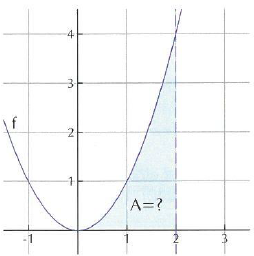
\includegraphics[width=0.3\textwidth]{images/x2_ausgang.png}}
	\end{wrapfigure}
	Wir möchten also die Fläche unter einer Kurve berechnen. Dazu betrachten wir die Funktion $f(x)=x^2$ und möchten dabei die eingeschlossene Fläche zwischen $a=0$ und $b=2$. Die Situation ist nebenan dargestellt. Weil die blau markierte Figur auf der einen Seite mit durch den Parabelbogen begrenzt ist, können wir ihren Flächeninhalt mit unseren bisherigen geometrischem Mittel nicht exakt berechnen. Daher möchten wir den Flächeninhalt näherungsweise berechnen und schrittweise verbessern. Die Idee, die wir verfolgen wollen, ist die Fläche in $n=4$ gleich breite, senkrechte Streifen zu zerlegen. Jeder dieser Streifen hat auf der $x$-Achse eine Breite von $\frac{1}{2}$. Die Höhe der Streifen wird in zwei verschiedenen Varianten berechnet.\vspace{10pt}\newline
	\begin{minipage}{0.8\linewidth}
		\textbf{Untersumme:}
		\center{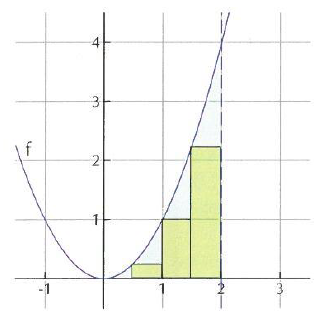
\includegraphics[width=0.7\textwidth]{images/x2_USumme4.png}}\newline
		Die Höhe jedes Rechtecks ist gleich dem \textbf{kleinstmöglichen} Funktionswert $f(x)$ in jedem Streifen. Berechnen wir also die Höhen der Rechtecke abhängig von der Funktion $f$:
		\begin{enumerate}[label=\ ]\begin{multicols}{2}
				\item $f(0)=$ \newline
				\item $f(0.5)=$
				\item $f(1)=$ \newline
				\item $f(1.5)=$
		\end{multicols}\end{enumerate}
	\end{minipage}
	\hfill
	\begin{minipage}{0.8\linewidth}
		\textbf{Obersumme:}
		\center{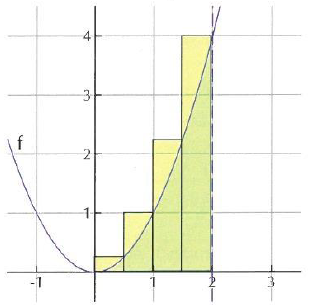
\includegraphics[width=0.7\textwidth]{images/x2_OSumme4.png}}\newline
		Die Höhe jedes Rechtecks ist gleich dem \textbf{grösstmöglichen} Funktionswert $f(x)$ in jedem Streifen. Im Unterschied zum ersten befinden sich die Höhen hier auf der rechten Seite.
		\begin{enumerate}[label=\ ]\begin{multicols}{2}
				\item $f(0.5)=$ \newline
				\item $f(1)=$
				\item $f(1.5)=$ \newline
				\item $f(2)=$
		\end{multicols}\end{enumerate}
	\end{minipage}
	\begin{minipage}{0.8\linewidth}
		Summieren wir nun alle Rechteckflächen, so erhalten wir:
		\begin{align*}
			U_4&=\lineortext{0.5\*0+0.5\*0.25+0.5\*1+0.5\*2.25}\\
			&=\lineortext{0+0.125+0.5+1.125=1.75}
		\end{align*}
	\end{minipage}
	\hfill
	\begin{minipage}{0.8\linewidth}
		Summieren wir nun alle Rechteckflächen, so erhalten wir:
		\begin{align*}
			O_4&=\lineortext{0.5\*0.25+0.5\*1+0.5\*2.25+0.5\*4}\\
			&=\lineortext{0.125+0.5+1.125+2=3.75}
		\end{align*}
	\end{minipage}\vspace{5pt}
	Zusammenfassend können wir also sagen, dass die blau eingefärbte Fläche mit den folgenden Ungleichungen angenähert werden kann. \[\lineortext{1.75} < A < \lineortext{3.75}\] Wir stellen aber auch fest, dass die Genauigkeit für diese Fläche noch sehr ungenau ist. Wir könnten versuchen, dies mit dem Durchschnitt beider Resultate schätzungsweise verbessern aber auch dies bietet nicht die zum Ziel gesetzte exakte Berechnung der Fläche.\newline
	Wir können aber ähnlich wie wir dies bereits bei mehreren Stellen schon gemacht haben die Anzahl der Rechtecke verdoppeln. Dabei wird die Breite der Rechtecke halbiert und und somit wird auch die Annäherung besser sein. Damit haben wir eine Breite der Rechtecke von $\frac{1}{4}$.
	\begin{minipage}{0.8\linewidth}
		\center{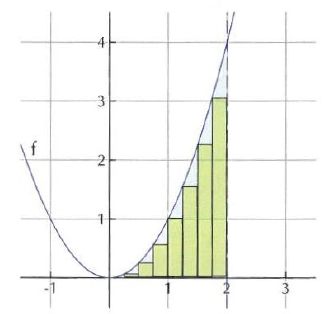
\includegraphics[width=0.7\textwidth]{images/x2_USumme8.png}}\newline
		Die Höhe der Rechtecke ist also:
		\begin{enumerate}[label=\ ]\begin{multicols}{2}
				\item $f(0)=0$
				\item $f(\frac{1}{4})=\frac{1}{16}$
				\item $f(\frac{1}{2})=\frac{1}{4}$
				\item $f(\frac{3}{4})=\frac{9}{16}$
				\item $f(1)=1$
				\item $f(\frac{5}{4})=\frac{25}{16}$
				\item $f(\frac{3}{2})=\frac{9}{4}$
				\item $f(\frac{7}{4})=\frac{49}{16}$
		\end{multicols}\end{enumerate}
		Die Summe alle Rechtecke kann wie folgt berechnet werden:
		\begin{align*}
			U_8&=\frac{1}{4}\*\left(0+\frac{1}{16}+\frac{1}{4}+\frac{9}{16}+1+\frac{25}{16}+\frac{9}{4}+\frac{49}{16}\right)\\
			&=2.1875\\
		\end{align*}
	\end{minipage}
	\hfill
	\begin{minipage}{0.8\linewidth}
		\center{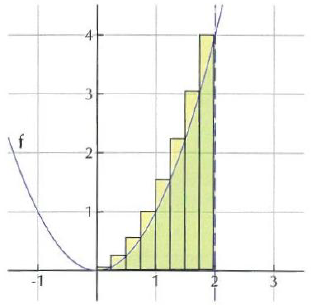
\includegraphics[width=0.7\textwidth]{images/x2_OSumme8.png}}\newline
		Die Höhe der Rechtecke ist also:
		\begin{enumerate}[label=\ ]\begin{multicols}{2}
				\item $f(\frac{1}{4})=\frac{1}{16}$
				\item $f(\frac{1}{2})=\frac{1}{4}$
				\item $f(\frac{3}{4})=\frac{9}{16}$
				\item $f(1)=1$
				\item $f(\frac{5}{4})=\frac{25}{16}$
				\item $f(\frac{3}{2})=\frac{9}{4}$
				\item $f(\frac{7}{4})=\frac{49}{16}$
				\item $f(2)=4$
		\end{multicols}\end{enumerate}
		Die Summe alle Rechtecke kann wie folgt berechnet werden:
		\begin{align*}
			O_8&=\frac{1}{4}\*\left(\frac{1}{16}+\frac{1}{4}+\frac{9}{16}+1+\frac{25}{16}+\frac{9}{4}+\frac{49}{16}+4\right)\\
			&=3.1875\\
		\end{align*}
	\end{minipage}
	Zusammenfassend sehen wir also, dass wir die Berechnung für die Fläche verbessern konnten und neu nur noch eine Ungenauigkeit von $1$ aufweist.\[2.1875<A<3.1875\]
	Natürlich können wir jetzt die die Anzahl Rechtecke erneut verdoppeln und so eine noch genauere Anschätzung erhalten. Wir sehen dann:\newline
	\begin{minipage}{0.8\linewidth}
		\begin{align*}
			n&=16:\qquad &&U_{16}=2.421875 \\
			n&=32:\qquad &&U_{32}=2.542968\ldots\\
			n&=64:\qquad &&U_{64}=2.604492\ldots\\
			n&=128:\qquad &&U_{128}=2.635498\ldots
		\end{align*}
	\end{minipage}
	\hfill
	\begin{minipage}{0.8\linewidth}
		\begin{align*}
			n&=16:\qquad &&O_{16}=2.921875\\
			n&=32:\qquad &&O_{32}=2.792968\ldots\\
			n&=64:\qquad &&O_{64}=2.729492\ldots\\
			n&=128:\qquad &&O_{128}=2.697998\ldots
		\end{align*}
	\end{minipage}\vspace{10pt}\newline
	Betrachten wir sowohl $U_n$ und $O_n$ als eine Folge und lassen $n$ nach unendlich gehen, was die Breite der Rechtecke immer kleiner werden lässt, so erhalten wir ein Resultat für die Fläche.
	\[A=\lim_{n\to\infty}U_n = \lim_{n\to\infty}O_n=\frac{8}{3}\]
	Um das Konzept zu festigen, folgen einige in Schwierigkeit aufbauende Aufgaben.

	\begin{aufgabe}
		Betrachte die Funktion $f(x)=x$ im Bereich $a=0$ und $b=1$.
		\begin{enumerate}[label=\alph*)]
			\item Teile das Intervall in $5$ gleich breite Teile und berechne die Fläche unter $f$ mithilfe der Ober- und Untersumme.
			\item Da $f$ eine lineare Funktion ist, sind wir in der Lage, die Fläche exakt berechnen. Vergleiche deine Lösung mit den Annäherungen aus $a)$.
		\end{enumerate}
	\end{aufgabe}
	\begin{aufgabe}
		Betrachte die Funktion $f(x)=\frac{1}{2}x+2$ im Bereich $a=1$ und $b=4$.
		\begin{enumerate}[label=\alph*)]
			\item Teile das Intervall in $5$ gleich breite Teile und berechne die Fläche unter $f$ mithilfe der Ober- und Untersumme.
			\item Die Anzahl der Rechtecke wurde bewusst mühsam gewählt, um dich zu zwingen, genau zu überlegen, wie breit ein Rechteck ist. Wie breit ist ein Rechteck, wenn wir die Breite abhängig von der Anzahl Rechtecke $n$ beschreiben wollen.
			\item Da $f$ eine lineare Funktion ist, sind wir in der Lage, die Fläche exakt berechnen. Vergleiche deine Lösung mit den Annäherungen aus $a)$.
		\end{enumerate}
	\end{aufgabe}
	\begin{aufgabe}
		Betrachte die Funktion $f(x)=\frac{1}{x}$ im Bereich $a=2$ und $b=4$.\newline
		\begin{minipage}{0.55\linewidth}
			\begin{enumerate}[label=\alph*)]
				\item Der Graph der Funktion fällt, deshalb überlege dir gut, was die Höhe der Rechtecke ist.
				\item Benutze $6$ Rechtecke, um die Ober- und Untersumme zu berechnen.
				\item Benutze das folgende \href{https://www.geogebra.org/m/vzjzrfdj}{Geogebra-Applet}\footnotemark, um deine Berechnungen zu überprüfen.
			\end{enumerate}
		\end{minipage}
		\hfill
		\begin{minipage}{0.4\linewidth}
			\centering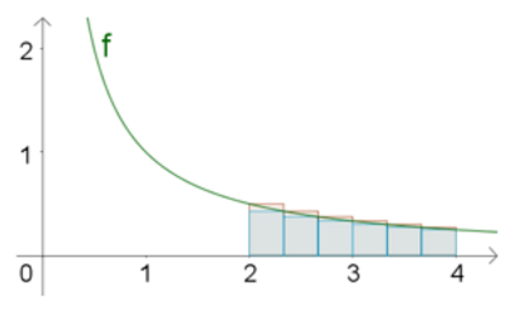
\includegraphics[scale=0.25]{images/aufg_OberUnter.png}
		\end{minipage}
	\end{aufgabe}
	\footnotetext{\url{https://www.geogebra.org/m/vzjzrfdj}}
	\begin{definition}[bestimmtes Integral]
		Das bestimmte Integral einer Funktion $f$ im Intervall $\left[a,b\right]$ entspricht der Fläche unter der Kurve im Intervall $\left[a,b\right]$ und ist der Grenzwert des Ober- bzw. Untersumme.
		\[\int_a^b f(x)\:\d{x}=\lim_{n\to\infty}U_n=\lim_{n\to\infty}O_n\]

		\textit{Sprich:} Integral $f(x)$ für $x$ von $a$ bis $b$\newline
		\textbf{TR:} menu $\to\:4\:\to\:3$
	\end{definition}
	\begin{enumerate}[label=\Alph*)]
		\item Spezialfall $a=b$:\newline Falls die beiden Grenze zusammenfallen, so ist die Breite der Rechtecke $\lineortext{\frac{b-a}{n}=0}$ und damit sind sowohl die Ober- als auch die Untersumme ebenfalls gleich $0$. Das heisst: \[\lineortext{\int_a^af(x)\:\d{x}=0}.\]
		\item Spezialfall $a>b$:\newline Falls $a$ grösser ist als $b$, so gilt für die Breite der Rechtecke $\lineortext{\frac{b-a}{n}<0}$ und damit ändert sich auch das Vorzeichen des Integrals
		\[\lineortext{\I_a^b f(x)\:\d{x} = -\int_b^a f(x)\:\d{x}}.\]
	\end{enumerate}
	\begin{aufgabe}
		Skizziere für die folgenden Funktionen den Graphen und markiere darin die gesuchte Fläche.
		\begin{enumerate}[label=\alph*)]\begin{multicols}{4}
				\item $\displaystyle\int_0^2 3x^2\:\d{x}$
				\item $\displaystyle\int_1^3 x^3\:\d{x}$
				\item $\displaystyle\int_2^4(x^2+3)\:\d{x}$
				\item $\displaystyle\int_1^3(x^2-4x)\:\d{x}$
				\item $\displaystyle\int_0^4 \sqrt{x}\:\d{x}$
				\item $\displaystyle\int_0^1 5x\sqrt{x}\:\d{x}$
				\item $\displaystyle\int_0^\frac{\pi}{2}\cos{x}\:\d{x}$
				\item $\displaystyle\int_1^\pi\sin{x}\:\d{x}$
		\end{multicols}\end{enumerate}
	\end{aufgabe}


\newpage
\section{Die Stammfunktion}
	\begin{definition}[Stammfunktion]
		Eine Funktion $F$ heisst Stammfunktion zu $f$, falls $F'=f$ gilt.
	\end{definition}
	Das heisst, die Ableitung der Stammfunktion ist die gegebene Funktion. Aus diesem Grund reduziert sich die Suche nach einer Stammfunktion auf das Problem der Umkehrung des Ableitens. Versuchen wir also einige Ableitungen umzudrehen.
	\begin{aufgabe}
		Suche für die folgenden Polynome $f$ eine Funktion $F$, deren Ableitung $F'=f$ ist.
		\begin{enumerate}[label=\alph*)]\begin{multicols}{3}
				\item $f(x)=x$
				\item $f(x)=x^2$
				\item $f(x)=x^3$
				\item $f(x)=x^n$
				\item $f(x)=3x^4+x^2$
				\item $f(x)=4x^5-6x^2$
		\end{multicols}\end{enumerate}
		Wir haben also bei $d)$ eine allgemeine Form für ein Polynom gefunden und gleich wie beim Ableiten kann auch hier summandenweise vorgegangen werden.
	\end{aufgabe}
	\begin{aufgabe}
		Suche auch für die folgenden speziellen Funktionen eine Stammfunktion zu finden.
		\begin{enumerate}[label=\alph*)]\begin{multicols}{3}
				\item $f(x)=\e^x$
				\item $f(x)=\sqrt{x}$
				\item $f(x)=\frac{1}{x}$
				\item $f(x)=\sin{x}$
				\item $f(x)=\cos{x}$
		\end{multicols}\end{enumerate}
	\end{aufgabe}
	\begin{aufgabe}
		\begin{enumerate}[label=\alph*)]
			\item Betrachte die Funktion $F_1(x)=4x^2+3$. Ist $F_1$ eine Stammfunktion von $f(x)=8x$?
			\item Betrachte die Funktion $F_2(x)=4x^2+12$. Ist $F_2$ eine Stammfunktion von $f(x)=8x$?
			\item Betrachte die Funktion $F_3(x)=4x^2+c$ für $c\in\R$. Ist $F_3$ eine Stammfunktion von $f(x)=8x$?
			\item Welches der obigen Funktionen ist nun die korrekte Lösung?
		\end{enumerate}
	\end{aufgabe}
	\begin{satz}
		Falls $F$ eine beliebige Stammfunktion von $f$ ist und $c\in\R$ eine konstante Zahl, dann ist jede Funktion der Form $F(x)+c$ eine Stammfunktion von $f$.
	\end{satz}\newpage
	\begin{notation}
		Das unbestimmte Integral einer Funktion $f$ ist die Menge aller Stammfunktionen $F$.\\ Schreibweisen:
		\[\int f(x)\:\d x \text{ oder } F(x)+c\]
	\end{notation}
	Die Rechenregeln für die Integrale sind im Grunde die gleichen wie fürs differenzieren. Ausgenommen davon sind die Produkt- und Quotientenregel.
	\begin{satz}[Rechenregeln]
		\begin{minipage}{0.4\linewidth}
			\begin{enumerate}
				\item Summe zweier Funktionen:
				\item Differenz zweier Funktionen:
				\item Multiplikation mit konstanten Faktor:
			\end{enumerate}
		\end{minipage}
		\hfill
		\begin{minipage}{0.55\linewidth}
			\begin{enumerate}[label=\ ]
				\item $\int(f(x)+g(x))\d{x}=\int f(x)\d{x}+\int g(x)\d{x}$
				\item $\int(f(x)-g(x))\d{x}=\int f(x)\d{x}-\int g(x)\d{x}$
				\item $\int\l\*f(x)\d{x}=\l\*\int f(x)\d{x}$, wobei $\l\in\R$
			\end{enumerate}
		\end{minipage}
	\end{satz}
	\begin{aufgabe}
		Bestimme die folgenden unbestimmten Integrale:
		\begin{enumerate}[label=\alph*)]\begin{multicols}{2}
				\item $\int(x^4+x^3+x^2+x+1)\d{x}$
				\item $\int 7\*\e^x\d{x}$
				\item $\int(4\*\sin{x}-3\*\cos{x})\d{x}$
		\end{multicols}\end{enumerate}
	\end{aufgabe}

\subsection*{Zusammenfassung}
	Fassen wir die gefundenen Stammfunktionen in einer übersichtlichen Tabelle zusammen. Wir gehen hier immer von der mittleren Spalte aus. Der Vorgang nach links heisst \glqq ableiten\grqq\: und nach rechts heisst \glqq integrieren\grqq. (vlg. Formelsammlung Seite $29-30$)
	\begingroup
	\renewcommand{\arraystretch}{1.5}
	\begin{table}[ht]
		\centering
		\begin{tabular}{p{2cm}|p{2cm}|p{3cm}|c}
			$f'$ & $f=F'$ & $F$ & Bedingung \\\hline
			$n\*x^{n-1}$ & $x^n$ & $\frac{1}{n+1}\* x^{n+1}+c$ & $n\in\Z\:\backslash\:\{-1\}$ \\
			$\frac{1}{2\sqrt{x}}$ & $\sqrt{x}$ & $\lineortext{\frac{2}{3}x^\frac{3}{2}+c}$ & \\
			$\exp{x}$ & $\exp{x}$ & $\lineortext{\exp{x}+c}$ & \\
			$\frac{1}{x}$ & $\ln{x}$ & $\lineortext{x\*\log{x}-x+c}$ & \\
			$\cos{x}$ & $\sin{x}$ & $\lineortext{-\cos{x}+c}$ & \\
			$-\sin{x}$ & $\cos{x}$ & $\lineortext{\sin{x}+c}$ & \\
			$\frac{1}{\cos{x}^2}$ & $\tan{x}$ & $-\ln{\cos{x}}+c$ & \\
			$\frac{a}{2\sqrt{a\*x}}$ & $\sqrt{a\*x}$ & $\frac{2}{3}\sqrt{a}\*x^\frac{3}{2}+c$ & $a>0$ \\
		\end{tabular}
	\end{table}
	\endgroup\newpage

\section{Der Hauptsatz der Differential und Integralrechnung}
	Wir stehen also vor einem Problem. Wir wissen, dass die Fläche unter einer Kurve mit Hilfe von Rechtecken angenähert werden kann. Leider ist dies aber extrem zeitaufwändig und oftmals auch algebraisch schwierig zu berechnen. Erstaunlicherweise ist die Lösung dieses Problems sehr einfach.
	\begin{satz}
		Gegeben ist eine Funktion $f$ im Intervall $\left[a,b\right]$ und eine beliebige Stammfunktion $F$ von $f$.\newline
		Dann  ist die Funktion \[A(x)=\int_a^x f(t)\d{t}\] eine Stammfunktion von $f$ und für die Fläche unter der Kurve gilt: \[\int_a^b f(x)\d{x}=\left[F(x)\right]_a^b=F(b)-F(a)\]
	\end{satz}
	\begin{beweis}
		\begin{wrapfigure}{r}{0.4\textwidth}
			\center{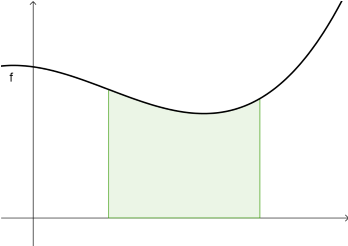
\includegraphics[width=0.3\textwidth]{images/flächenfunktion.png}}
		\end{wrapfigure}
		Die Funktion \[A(x)=\int_a^x f(t)\d{t}\] beschreibt die Fläche unter dem Graph von $f$ zwischen $a$ und $x$. Im ersten Schritt müssen wir jedoch überprüfen, ob $A(x)$ eine Stammfunktion von $f$ ist. Dabei genügt es zu zeigen, dass $A(x)$ abgeleitet gleich $f$ ist.
		\vspace{6cm}\newline
		Das heisst also, $A(x)$ ist eine Stammfunktion von $f$ und es gilt: \[A(x)=\int_a^x f(t)\d{t} = F(x)+c.\] Zum Schluss wäre es jedoch schön, wenn wir herausfinden, welchen Wert der Parameter $c$ erhält. Dazu nutzen wir den Spezialfall $a=b$, in dem die Grenzen aufeinander fallen.
		\vspace{4cm}\newline
		Damit folgt also die Behauptung \[\int_a^b f(x)\d{x}=F(b)-F(a).\]\flushright{$\blacksquare$}
	\end{beweis}
	\begin{beispiel}
		Betrachte die Funktion $f(x)=x^2$. Analog zum Vorgang mit der Ober- und Untersumme wollen wir die Fläche unter der Kurve zwischen $a=0$ und $b=2$ berechnen.
		\vspace{5pt}\newline\karos{6}
	\end{beispiel}
	\begin{aufgabe}
		\begin{enumcols}[4]
			\item $\int_0^2 3\*x^3\d{x}$
			\item $\int_1^3 x^3\d{x}$
			\item $\int_2^4\left(x^2+3\right)\d{x}$
			\item $\int_1^3\left(x^2-4x\right)\d{x}$
			\item $\int_0^4\sqrt{x}\d{x}$
			\item $\int_0^1 5x\*\sqrt{x}\d{x}$
			\item $\int_0^{\frac{\pi}{2}}\cos{x}\d{x}$
			\item $\int_0^\pi\sin{x}\d{x}$
			\item $\int_1^2\left(2x-\frac{2}{x}\right)\d{x}$
			\item $\int_1^3\left(4x-\frac{3}{x}+\frac{2}{x^2}\right)\d{x}$
			\item $\int_1^2\left(\frac{4}{x}+\frac{5}{x^2}+\frac{6}{x^3}\right)\d{x}$
			\item $\int_1^2\left(\e^x+\frac{1}{x}\right)\d{x}$
		\end{enumcols}
	\end{aufgabe}


\newpage
\section{Anwendungen des Integrals}
	Im Folgenden werden wir einige Eigenschaften des Integrals im Zusammenhang mit Flächenberechnungen kennenlernen.
\subsection{Fläche zwischen Graph und $x$-Achse}
	\vspace{5pt}
	\begin{aufgabe}
		Betrachte die Funktion $f(x)=\frac{1}{4}x^3-3x^2+8x$ im Intervall $\left[0,8\right]$.
		\begin{table}[H]
			\centering
			\begin{tabular}{p{7cm} c}
				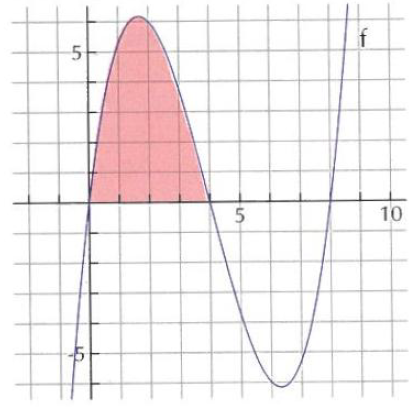
\includegraphics[scale=0.3]{images/flächePosNeg1.png} & 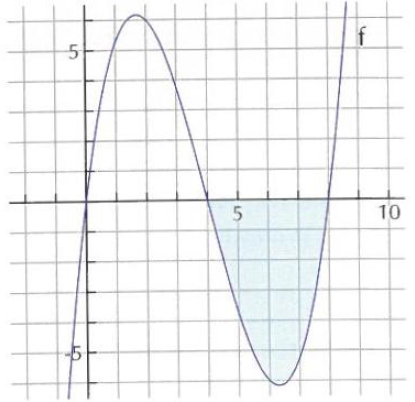
\includegraphics[scale=0.3]{images/flächePosNeg2.png} \\
				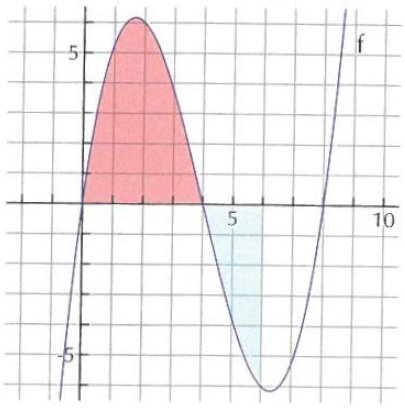
\includegraphics[scale=0.3]{images/flächePosNeg3.png} & 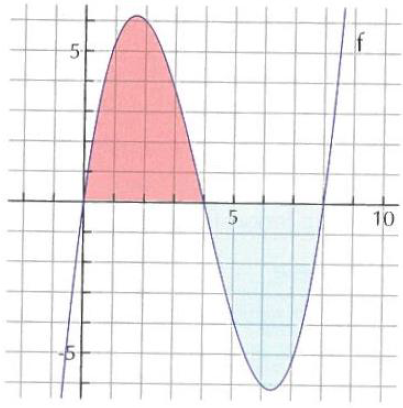
\includegraphics[scale=0.3]{images/flächePosNeg4.png}
			\end{tabular}
		\end{table}
		\begin{enumerate}[label=\alph*)]
			\item Berechne für jeden oben abgebildeten Graphen die eingezeichnete Fläche.\vspace{5pt}\newline\karos{6}
			\item Erkläre das Problem, welches du feststellst.\vspace{5pt}\newline\karos{2}
			\item Suche nach einer möglichen Lösung und beschreibe dein Lösungsweg möglichst genau. \textit{Tipp: Nullstellen}\vspace{5pt}\newline\karos{2}
		\end{enumerate}
	\end{aufgabe}
	\begin{algo}
		Das Verfahren zur Berechnung des Flächeninhalts $A$ zwischen dem Graphen einer Funktion und der $x$-Achse kann in folgende $3$ Schritte aufgeteilt werden.
		\begin{enumerate}
			\item \lineortext{Berechne alle Nullstellen $x_1,\ldots,x_n$ von $f$ im Intervall $\left[a,b\right]$}
			\item \lineortext{Berechne die Beträge aller Integrale zwischen den Nullstellen}
			\item \lineortext{Summiere alle Teilresultate:}\[\lineortext{A=\abs*{\int_a^{x_1}f(x)\d{x}}+\ldots+\abs*{\int_{x_n}^b f(x)\d{x}}}\]
		\end{enumerate}
	\end{algo}
	\begin{aufgabe}
		Zeige, dass die durch die Gleichung gegebene Funktion $f$ im Innern des Intervalls $\left[a,b\right]$ genau eine Nullstelle hat. Berechne danach den Flächeninhalt $A$.
		\begin{enumcols}[2]
			\item $f(x)=x^2-6x+5;\quad a=2,b=8$
			\item $f(x)=2\e^x-1;\quad a=-2,b=1$
			\item $f(x)=\frac{1}{2}x^3-2x^2-\frac{7}{2}x+5;\quad a=-1,b=3$
			\item $f(x)=\cos{3x};\quad a=0,b=\frac{\pi}{2}$
		\end{enumcols}
	\end{aufgabe}
	\begin{aufgabe}
		Berechne die vom Graphen und der $x-$Achse eingeschlossene Fläche.
		\begin{enumcols}[3]
			\item $f(x)=-x^2+4x-3$
			\item $f(x)=x+\frac{1}{x}-4$
			\item $f(x)=-x^4-x^3+4x^2+4x$
		\end{enumcols}
	\end{aufgabe}
	\begin{aufgabe}
		Die Parabel $p:y=ax-x^2$ schliesst im 1. Quadranten mit der $x-$Achse eine Fläche vom Inhalt $A=36$ ein. Berechne den Parameter $a$.
	\end{aufgabe}

\subsection{Fläche zwischen zwei Graphen}
	Mithilfe der Überlegungen aus dem letzten Abschnitt wollen wir versuchen eine Möglichkeit zu finden, die Fläche zwischen den Graphen zweier Funktionen $f$ und $g$ zu berechnen. Hier ist natürlich wichtig, dass es sich um eine abgeschlossene Fläche handelt.
	\begin{aufgabe}
		Betrachte die Funktionen $f(x)=-x^2+3x+3$ und $g(x)=x^2-4x+6$ im folgenden \href{https://www.geogebra.org/m/gfdvryzw}{Geogebra-Applet}\footnotemark.
		\begin{enumerate}[label=\alph*)]
			\item Wie lässt sich die Länge der senkrechten orangen Strecken mathematisch beschrieben.\vspace{5pt}\newline\karos{1}
			\item Verschiebe nun die Fläche, sodass sie direkt über der $x-$Achse liegt. Was beschreibt diese Funktion?\vspace{5pt}\newline\karos{1}
			\item Wir definieren die Differenzfunktion $f(x)-g(x)$. Welche Fläche wir nun von dieser Differenzfunktion und der $x-$Achse eingeschlossen?\vspace{5pt}\newline\karos{1}
			\item Schliesse daraus eine Formel zur Berechnung der Fläche zwischen den beiden Graphen und wende sie auf dieses Beispiel an.\vspace{5pt}\newline\karos{5}
		\end{enumerate}
	\end{aufgabe}
	\footnotetext{\url{https://www.geogebra.org/m/gfdvryzw}}
	\begin{algo}
		Das Verfahren zur Berechnung der Fläche zwischen zwei Graphen kann ebenfalls in $3$ Schritte beschrieben werden:
		\begin{enumerate}
			\item \lineortext{Berechne alle Schnittstellen von $f$ und $g$ im Intervall}
			\item \lineortext{Berechne die Beträge aller Teilintegrale der Differenzfunktion}
			\item \lineortext{Summiere die Teilresultate:}\[\lineortext{A=\abs*{\int_a^{s_1}\left(f(x)-g(x)\right)\d{x}}+\ldots+\abs*{\int_{s_n}^b \left(f(x)-g(x)\right)\d{x}}}\]
		\end{enumerate}
	\end{algo}
	\begin{aufgabe}
		Berechne die Fläche zwischen den Graphen der beiden Funktionen $f$ und $g$.
		\begin{enumerate}[label=\alph*)]
			\item $f(x)=x^3-5x^2+6x$, $g(x)=x^3-7x^2+12x$
			\item $f(x)=\frac{-1}{10}x^2+2$, $g(x)=x-1$, $\left[-1,2\right]$
			\item $f(x)=(-x)^{-2}$, $g(x)=x^2$, $\left[-2,4\right]$
			\item $f(x)=\sin{x}$, $g(x)=1-\sin{x}$, $\left[0,\frac{5\pi}{6}\right]$
		\end{enumerate}
		\textit{Tipp:} Es hilft die beiden Funktion zur Kontrolle in TR zu zeichnen.
	\end{aufgabe}

\subsection{Volumen eines Rotationskörpers}
	Bis anhin haben wir die Integralrechnung durchwegs zur Bestimmung von Flächeninhalten verwendet. Wir wollen dies nun erweitern und zeigen, dass wir mit unseren Kenntnissen auch \textbf{Volumen} bestimmen können:
	\begin{definition}
		Rotiert eine Fläche, die in einem Intervall $[a,b]\subset\R$ zwischen dem Graphen einer Funktion $f$ und der $x-$Achse liegt, um die $x-$Achse, so erzeugt die Fläche bei ihrer Umdrehung um $360^\circ$ einen symmetrisch zur $x-$Achse liegenden \textbf{Rotationskörper}.
	\end{definition}
	\begin{aufgabe}
		Untersuchen Sie den folgenden Rotationskörper im Intervall $[1,5]$ und lösen Sie die untenstehenden Teilaufgaben.
		\begin{enumerate}[label=\alph*)]
			\item Berechnen Sie das Volumen des abgebildeten Zylinders.
			\begin{figure}[H]
				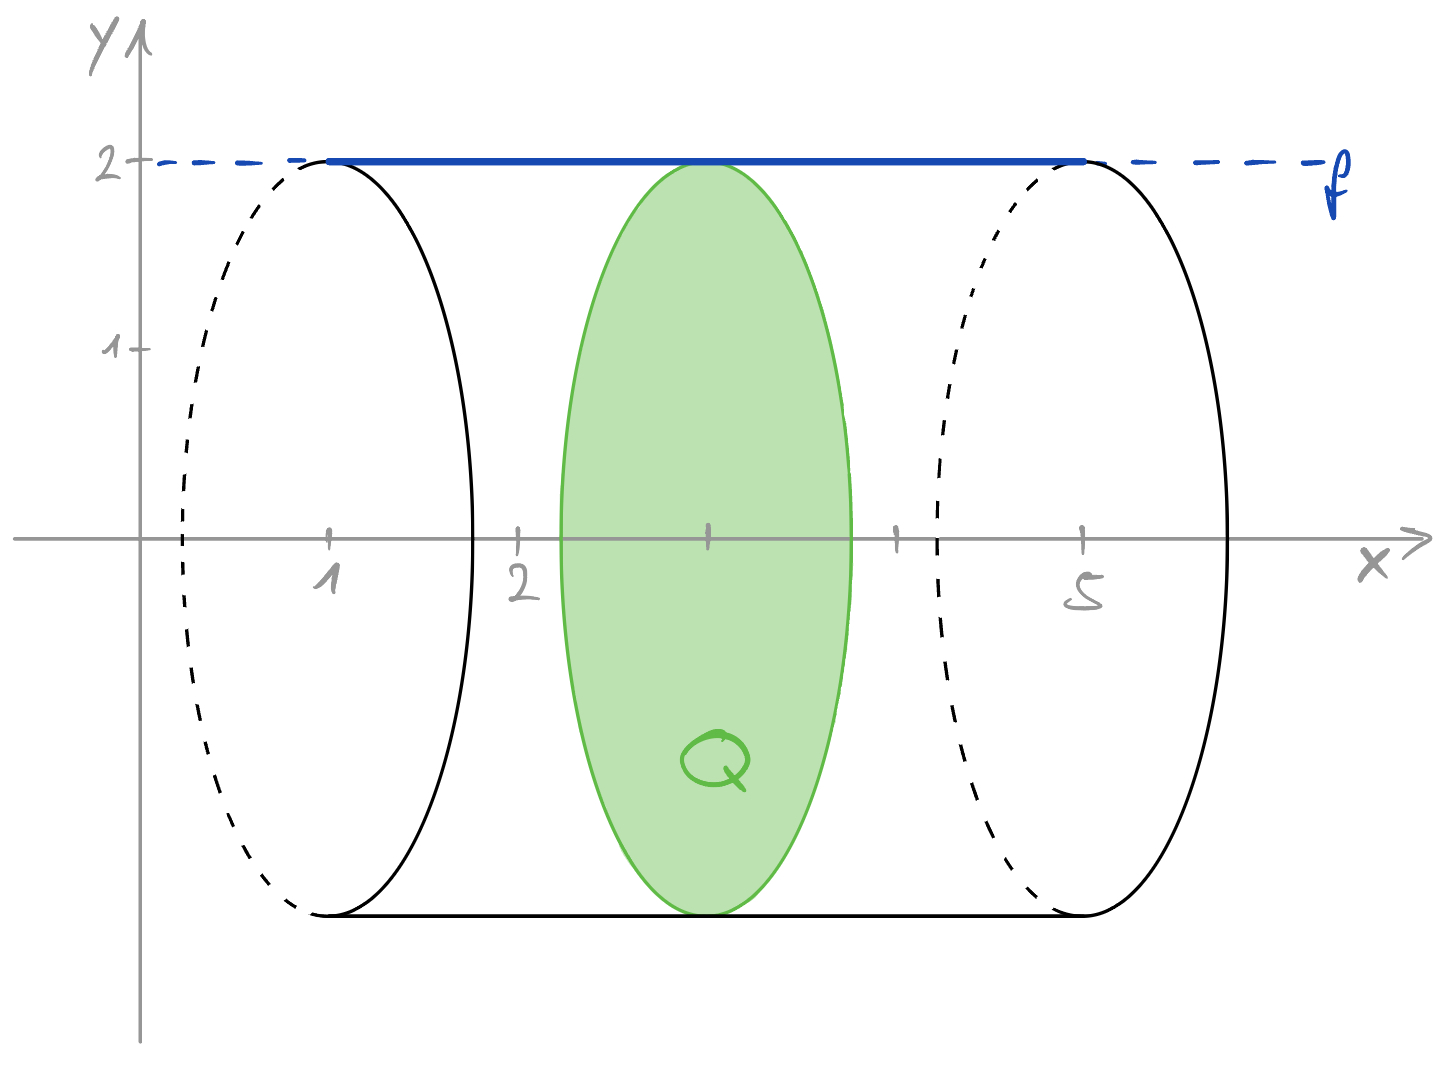
\includegraphics[scale=0.1]{images/zylinder.jpeg}
			\end{figure}
			\item Wir sehen also, dass ein Zylinder als Rotationskörper einer konstanten Funktion aufgefasst werden kann. Drücken Sie das Volumen des Zylinders in Abhängigkeit einer konstanten Funktion $f(x)$ aus.
		\end{enumerate}
		\vspace{5pt}\karos{2.5}\newpage
		\begin{enumerate}[label=\alph*)]
			\setcounter{enumi}{2}
			\item Berechnen Sie das Volumen des abgebildeten Kreiskegels mit Radius $r=5$ und Höhe $h=12$.
			\begin{figure}[H]
				\begin{tikzpicture}[cross/.style={draw, cross out, minimum size=2*(#1-1pt), inner sep=0pt, outer sep=0pt}, x=7.5mm, y=7.5mm,
					>=latex,   %Voreinstellung für Pfeilspitzen
					font= \footnotesize, scale=0.8]
					%Raster zeichnen
					\draw [color=gray!50]  [step=7.5mm] (-1.3,-5.3) grid (14.8,5.8);
					% Achsen zeichnen
					\draw[->,thick] (-1.3,0) -- (14.8,0) node[right, below] {\normalsize $x$};
					\draw[->,thick] (0,-5.3) -- (0,5.8) node[above, left] {\normalsize $y$};
					% Achsen beschriften
					\foreach \x in {-1,1,2,...,14} \draw (\x,-.1) -- (\x,.1) node[below=4pt] {$\x$};
					\foreach \y in {-5,...,-1,1,2,...,5} \draw (-.1,\y) -- (.1,\y) node[left=4pt] {$\y$};
					% Besserer Ursprung
					\draw[color=black] (0pt,-7pt) node[right] {$0$};
					%Funktionen zeichnen:
					\clip(-0.8,-5.1) rectangle (14.1,5.3); %Bildbereich
					\draw[blue, smooth, domain=-9:15] plot (\x, {5/12*\x}) node[] {};
					\draw[black, smooth, domain=0:12] plot (\x, {-5/12*\x}) node[] {};
					\draw[black] (12,0) ellipse (10mm and 37.5mm);
					%Beschriftung
					\node[blue]  at (11,5) {\normalsize$f$};
				\end{tikzpicture}
			\end{figure}
		\end{enumerate}
	\end{aufgabe}
	Wir haben nun also zwei einfache Beispiele gesehen. Da wir bis jetzt aber immer geradlinig begrenzte Flächen hatten, konnten wir die bekannten Volumenformel verwenden. Deshalb stellt sich nun natürlich die Frage, wie kann das Vorgehen auf krummlinige Flächen erweitert werden?
	\begin{beispiel}
		Die Fläche zwischen dem Graphen der Funktion $f(x)=4x-x^2$ und der $x-$Achse rotiert um die $x-$Achse. Berechnen Sie das Volumen des Rotationskörpers.\vspace{7pt}\newline
		\begin{minipage}{0.47\linewidth}
			\begin{tikzpicture}[cross/.style={draw, cross out, minimum size=2*(#1-1pt), inner sep=0pt, outer sep=0pt}, x=10mm, y=10mm,
				>=latex,   %Voreinstellung für Pfeilspitzen
				font= \footnotesize, scale=0.9]
				%Raster zeichnen
				\draw [color=gray!50]  [step=10mm] (-0.6,-1.6) grid (4.6,4.6);
				% Achsen zeichnen
				\draw[->,thick] (-0.8,0) -- (4.8,0) node[right, below] {\normalsize $x$};
				\draw[->,thick] (0,-1.8) -- (0,4.8) node[above, left] {\normalsize $y$};
				% Achsen beschriften
				\foreach \x in {1,2,...,4} \draw (\x,-.1) -- (\x,.1) node[below=4pt] {$\x$};
				\foreach \y in {-1,1,2,...,4} \draw (-.1,\y) -- (.1,\y) node[left=4pt] {$\y$};
				% Besserer Ursprung
				\draw[color=black] (0pt,-7pt) node[right] {$0$};
				%Funktionen zeichnen:
				\clip(-0.6,-1.6) rectangle (4.6,4.6); %Bildbereich
				\draw[blue,domain=-0.5:4.5,samples=100] plot (\x, {4*\x-\x*\x});
				%Beschriftung
				\node[blue]  at (4.4,-0.8) {\normalsize$f$};
			\end{tikzpicture}

			Fläche unter dem Graphen von $f$:
			\begin{align*}
				A_4&=\sum_{i=1}^4 f(x_i)\*\Delta x\\
				&\ \\
				&\ \\
			\end{align*}
		\end{minipage}
		\hfill\vline\hfill
		\begin{minipage}{0.47\linewidth}
			Volumen von Rotationskörper:
			\vspace{9.5cm}
		\end{minipage}
		\begin{minipage}{0.47\linewidth}
			Fläche unter dem Graphen von $f$:
			\begin{align*}
				A&=\lim_{n\to\infty}A_n\\
				&=\lim_{n\to\infty}\sum_{i=1}^n f(x_i)\*\Delta x\\
				&=\int_0^{12} f(x)\d{x}\\
				&\ \\
				&\ \\
				&\ \\
				&\ \\
				&\ \\
				&\ \\
				&\ \\
				&\
			\end{align*}
		\end{minipage}
		\hfill\vline\hfill
		\begin{minipage}{0.47\linewidth}
			Volumen von Rotationskörper:
			\vspace{8.6cm}
		\end{minipage}
	\end{beispiel}
	\begin{satz}
		Sei $f$ eine im Intervall $\left[a,b\right]$ stetige und nicht negative Funktion. Rotiert die Fläche zwischen dem Graphen von $f$ und der x-Achse im Intervall $[a,b]$ um die x-Achse, so gilt für das Volumen des erzeugten Rotationskörper:
		\[ V = \lineortext{\quad\pi \* \int_a^b \left(f(x)\right)^2 \d{x}\quad}\]
	\end{satz}
	Zusätzliche Infos zum Grenzwertprozess: \url{https://www.geogebra.org/m/tVDqQzvP}
	\begin{aufgabe}
		Die Fläche zwischen der $x-$Achse und der Funktion $f$ rotiert um die $x-$Achse. Welches Volumen hat der entstehende Rotationskörper?
		\begin{enumcols}[2]
			\item $f(x)=-x^2+4$
			\item $f(x)=3x-\frac{1}{2}x^2$
			\item $f(x)=\left(x^2-1\right)^2$
			\item $f(x)=x^3-3x^2$
		\end{enumcols}
	\end{aufgabe}
	\begin{aufgabe}[für die Schnellen]
		\begin{minipage}{0.6\linewidth}
			Das abgebildete Fass hat ein Parabelförmig gebogenes Daubenprofil. Der Mathematiker und Astronom \textbf{Johannes Kepler ($1571-1630$)} behauptete, das Volumen eines solchen Fasses wird mit der folgenden Formel berechnet:
			\[V=\frac{h\*\pi}{15}\left(8R^2+4Rr+3r^2\right).\] Beweise diese Formel.
		\end{minipage}
		\hfill
		\begin{minipage}{0.35\linewidth}
			\begin{figure}[H]
				\centering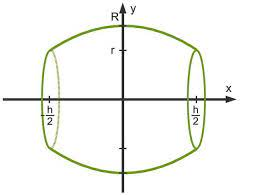
\includegraphics[scale=0.5]{images/keplerfass.jpeg}
			\end{figure}
		\end{minipage}
	\end{aufgabe}\newpage
	\begin{beispiel}
		Gabriels Horn
	\end{beispiel}

\subsection{Uneigentliche Integrale}
	tbd %Skript-Atchu --> PDF/LATEX


\newpage
\subsection*{History}
\begin{table}[H]
	\centering
	\begin{tabular}{|p{13mm}|p{20mm}|p{30mm}|p{70mm}|}\hline
		%\multicolumn{4}{|l|}{History}\\\hline
		Version & Datum & Person & Bemerkung \\\hline
		$1.0$ & 02.04.2025 & Jonas Guler & Kapitel erstellt \\\hline
		$1.1$ & ToDo & Jonas Guler & Rotationsvolumen überarbeiten, uneigentliche Integrale hinzufügen \\\hline
	\end{tabular}
\end{table}

\end{document}